\section{Molecular Networks}
\todo{order of subsections, update content correctly}

\todo[inline]{EFMs and extreme rays}

\subsection{Genome-Scale Metabolic Models}
\todo[inline]{GEMs}
\todo[inline]{research question}
\todo[inline]{computational systems biology}
\todo[inline]{differences between the differential equation models and FBA}

\subsection{Mathematical Representation}
A hypergraph $\mathscr{H}$ is defined by its set of vertices $\mathscr{V}$ and set of hyperedges $\mathscr{E}$. A hyperedge is a pair $E= (H,T)$ of disjoint subsets of $\mathscr{V}$, where $H$ denotes the vertices in the head and $T$ the vertices in the tail \cite{gallo_directed_1993}.

\todo[inline]{explain internal and external}

A metabolic network $\mathcal{N}$ can be represented as by the tuple ($\mathcal{M}, \mathcal{R}, S, l, u$), where $\mathcal M$ is the set of internal metabolites and $\mathcal{R}$ is the set of reactions. The hypergraph is stored in the stoichiometric matrix $S \in \mathbb{R}^{m\times n}$, where $m$ is the number of internal metabolites and $n$ is the number of reactions, including internal reactions $\mathcal{I}$ and exchange reactions $\mathcal{E}$. Exchange reactions are reactions where nutrition is taken up or where a product is discarded by the cell. 
A subset of internal reactions are \textit{currency exchange} reactions, where the currency of metabolites between different sub-networks in the cell is exchanged, such as ATP-hydrolysis. \todo[inline]{ATP hydrolysis}

The columns of $S$ correspond to the reactions in the network and the entries are the stoichiometric coefficients for each reaction and capture the mass balance for each metabolite. A negative coefficient indicates that a metabolite is consumed and in the tail of the hyperedge. Vice versa, if the coefficient is positive, the metabolite is produced and in the head of the hyperedge.
The matrix $S_\mathcal{I}$ is the submatrix of $S$ that contains the columns of internal reactions only. 

The stoichiometric matrix $S$ relates the flux vector $v$ to the change in metabolite concentration: $\frac{dx}{dt} = Sv$ \cite{noor_removing_2018}. 

$l$ and $u$ capture the lower and upper bounds for all reactions. If the direction of a reaction is determined by the bounds, the reaction is said to be \textit{irreversible}. Otherwise it is \textit{reversible}.

\begin{figure}[h!]
    \centering
    \caption{simplified molecular network}
    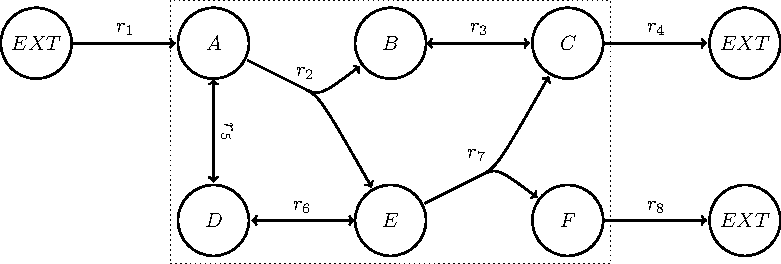
\includegraphics[width=0.8\textwidth]{Images/tikz_graphs_model_with_hyperarcs.pdf}
    \label{fig:simple_model}
\end{figure}

\todo[inline]{fix labels}

\cref{fig:simple_model} shows a simplified molecular network with three exchange reactions $\{r_1, r_4, r_8\}$ and five internal reactions $\{r_2, r_3, r_5, r_6\}$. The set of internal metabolites is $\{A, B, C, D, E, F\}$. The set of reversible reactions is $\{r_5, r_6, r_3\}$ and the set of irreversible reactions $\{r_1, r_2, r_4, r_7, r_8\}$. If no other bounds are known, all irreversible reactions have to be greater or equal to zero. The corresponding stoichiometric matrix $S$ is:

\begin{equation*}
    S = \begin{pmatrix}
        1 & -1 & 0 & 0 & -1 & 0 & 0 & 0\\
        0 & 1 & -1 & 0 & 0 & 0 & 0 & 0\\
        0 & 0 & 1 & -1 & 0 & 0 & 1 & 0\\
        0 & 0 & 0 & 0 & 1 & -1 & 0 & 0\\
        0 & 1 & 0 & 0 & 0 & 1 & -1 & 0\\
        0 & 0 & 0 & 0 & 0 & 0 & 1 & -1\\
    \end{pmatrix}
\end{equation*}


\subsection{Extreme Pathways}
There are three types of extreme pathways: \textit{primary systemic pathways} (Type \rom{1}), \textit{futile cycles} (Type \rom{2}) and \textit{internal cycles} (Type \rom{3}). \todo{thermodynamic feasibility} 
Primary systemic pathways are pathways where at least one primary exchange flux is active. These pathways are wanted steady-state flux solutions. Internal cycles are pathways where non of the exchange reactions are used and are not wanted as steady-state flux solutions. Futile cycles are pathways where none of the primary exchange fluxes are active, but at least one currency exchange flux is active. Looking at ATP-hydrolysis... \todo[inline]{hydrolysis} Energy reducing cycles are biologically feasible and should be allowed solutions, whereas energy generating cycles (EGCs) are not wanted as solutions. EGCs are problematic as they can lead to solutions that have a better objective value than when restricting the use of EGCs. One possibility to prevent EGCs is by restricting the directionality of the reaction. 

\cite{noor_removing_2018}
\todo[inline]{visualisation}

\subsection{Thermodynamic Feasibility}
\todo[inline]{first and second law of thermodynamics}

The second law of thermodynamics applied to enzyme-catalysed reactions states that: 
\begin{equation}
    \Delta \mu = \Delta \mu \degree + RT \sum_{i} v_i \mathrm{ln} (c_i)
    \label{Eq:lawOfThermodynamics}
\end{equation}
\todo{R is a thermodynamic constant and T a temperature in Kelvin, elementwise log}
where $\Delta \mu_i$ is the change of Gibbs free energy for reaction $i$. $R$ is the gas and $T$ is the energy constant. $c_i$ is the concentration of metabolite $i$ and $v_i$ the stoichiometric coefficient. $\Delta \mu \degree$ is the standard chemical potential. 

In matrix notation, we have:

\begin{equation}
    \Delta \mu = \Delta \mu \degree + RT S \tran \mathrm{ln}(c)
\end{equation}

\todo{which formula to use}
\todo[inline]{Kirchoff}
\todo[inline]{thermo feasibility of extreme pathways}

It follows from \cref{Eq:lawOfThermodynamics} that $\forall i : v_i = 0 \lor sign(v_i) = - \text{sign}(\Delta \mu_i)$ \cite{noor_removing_2018}

\subsection{Enzyme Kinetics}

\subsection{Optimization for Molecular Networks}
Once a mathematical representation of a model is available, the question is which flows of metabolites are possible and likely to occur in an organism. Constraint-Based Reconstruction and Analysis (COBRA) are methods to analyse the set of possible flux distributions mathematically. The flow is represented by vector $v$, where $v_i$ indicates the units of flow through reaction $i$. 

COBRA methods use context-specific constraints such as reaction flux bounds, mass conservation and steady-state assumption \cite{cobrapy}. The flux through a reaction is limited and therefore lower bounded by vector $l$ and upper bounded by vector $u$. \todo{write vectors correctly, bold?} Mass balance is captured in the stoichiometry of reaction and products in a reaction. Additionally, a realistic flux should respect the steady-state assumption $Sv=0$. This constraint ensures a balance of the produced and consumed metabolite concentration. \todo{strong assumption?}  
These constraints reduce the solution space of feasible flux distributions, however usually there exist multiple valid flows. The solution space is a polytope defined by convex basis vectors which is the set of extreme pathways. 

One method to analyse the set of possible flows is to add an objective function $c$ and find a distribution $v*$ that optimizes it. A commonly used objective function is the maximization of growth. Growth can be incorporated into the stoichiometric matrix $S$ by adding an extra column where the coefficients indicate the contribution to growth.  \cite{FBA}

\todo[inline]{variations of COBRA}
Several COBRA methods relevant for this thesis are explained below.

\todo[inline]{link to mathematical optimization}
\todo[inline]{visualization of cobra methods}

\subsubsection{Flux Balance Analysis}
The most basic COBRA method is flux balance analysis (FBA) as shown in \cref{Eq:fba}. An optimal solution $v*$ to an FBA model, is a flux distribution maximizing a biological linear objective which respects steady-state constraints and bound constraints.

\begin{maxi!}
  {\scriptstyle v}{c\tran v}{\text{\textbf{FBA:}} \label{Eq:fba}}{}
    \addConstraint{Sv=0} 
    \addConstraint{l \leq v \leq u}
\end{maxi!}

where $c \in \mathbb{R}^n$ determines the linear objective function of the FBA. The structure of the network is captured in the stoichiometric matrix $S$.The fluxes $v \in \mathbb{R}^n$ are bounded by $l,u \in \mathbb{R}^n$. \cref{Eq:fba}(b) ensures the steady-state of the metabolite concentration. \todo{ref subequation}

\todo[inline]{runtime}
\todo[inline]{example} 

A solution to FBA can be a convex combination of primary systematic pathways, futile cycles and internal cycles. To prevent biologically implausible futile cycles, the directionality is restricted with the bound constraints \cref{Eq:fba} (c). Internal cycles are biologically not realistic, but are part of the solution space, posing a major drawback to FBA solutions. 

\begin{figure}[h!]
    \caption{simple model with internal loop}
    \centering
    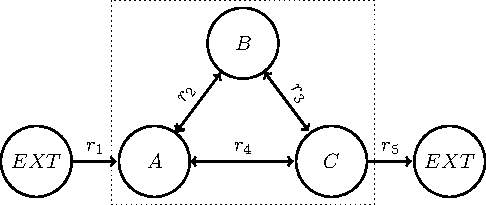
\includegraphics[width=0.8\textwidth]{Images/tikz_graphs_one_loop.pdf}
    \label{fig:loop}
\end{figure}
\todo[inline]{give example for infeasible solution, specify bounds etc}

\subsubsection*{Removing Internal Cycles}
\todo{rephrase section}
Linear Program that returns a thermodynamically feasible flux $v$ for a given flux $v^{(0)}$ \cite{desouki_cyclefreeflux_2015-1} if the reactions contained in a loop are allowed to be zero and if the objective does not depend on a reaction which is contained in a loop, and if the model does not contain energy-generating cycles \cite{noor_removing_2018}:

\begin{mini!}
    {\scriptstyle v}{\sum_i |v_i| = \sum_{i: v_i^{(0)} > 0} v_i - \sum_{i: v_i^{(0)} < 0} v_i}{\label{Eq:CycleFreeFlux}}{} 
    \addConstraint{Sv=0} 
    \addConstraint{{c\tran v} = {c\tran v}^{(0)}}
    \addConstraint{0 \leq v_i \leq v_i^{(0)} \quad \text{for $i$ with $v_i^{(0)} \geq 0$}}
    \addConstraint{v_i^{(0)} \leq v_i \leq 0 \quad \text{for $i$ with $v_i^{(0)} < 0$}}
    \addConstraint{v_i = v_i^{(0)} \quad \forall i \in \mathcal{E}}
\end{mini!}

Assuming that no reaction in a loop is maximized in the objective and such reactions are allowed to carry zero flux, 
solving the LP for a given FBA solution, provides another test for thermodynamic feasibility: $v^{(0)}$ is thermodynamically feasible if $v=v^{(0)}$, where $v$ is the solution to \eqref{Eq:CycleFreeFlux}.
And in that case \eqref{Eq:CycleFreeFlux} can be used to enumerate thermodynamically infeasible cycles.  

\todo[inline]{counter example}

\subsubsection{Thermodynamic Flux Balance Analysis}
One method that integrates thermodynamic data to get solutions that are thermodynamically feasible is thermodynamic flux balance analysis (TFBA). 

\begin{maxi!}
  {\scriptstyle v, a, x, \mu}{c\tran v}{\text{\textbf{TFBA:}} \label{Eq:tfba}}{}
    \addConstraint{Sv=0} 
    \addConstraint{l \leq v \leq u}
    \addConstraint{0 \leq Ma-v \leq M}
    \addConstraint{\epsilon \leq Ma + \mu \leq M - \epsilon}
    \addConstraint{\mu = \Delta \mu + RT * S_{INT} \tran x}
    \addConstraint{\mathrm{ln}(b^L) \leq x \leq \mathrm{ln}(b^U)}
    \addConstraint{a_i \in {0,1}}
\end{maxi!}

where the linear objective function \cref{Eq:tfba}(a), the steady-state constraints \cref{Eq:tfba}(b) and the bound constraints \cref{Eq:tfba}(c) \todo{equation ref layout} are exactly the FBA model \cref{Eq:fba}. \cref{Eq:tfba} (d) and (e) ensure that the second law of thermodynamics holds: $\forall i : v_i = 0 \lor sign(v_i) = - \text{sign}(\Delta \mu_i)$\todo{text in math mode}. $M$ is a large constant that does not restrict the size of $v$ and $\mu$. The binary variables $a$ indicate the direction of v: if $v_i>0 \implies a_i=1$ and if $v_i<0 \implies a_i=0$. If $a_i=1$, $v_i$ is zero or positive as $-M \leq -v_i \leq M$ holds. In that case, $\mu$ is negative as $\epsilon - M \leq \mu \leq - \epsilon$. If $a_i=0$, $0 \leq -v_i \leq M$ holds and the flux $v_i$ is zero or negative. $\mu$ is positive as $\epsilon \leq \mu \leq M - \epsilon$.
$x$ is the vector of metabolite concentrations which is bound by $\mathrm{ln}(b^L)$ and $\mathrm{ln}(b^U)$. 
\todo[inline]{write about (2f)}
\todo{variables do not match names in ll FBA}

\cite{noor_removing_2018}

\todo[inline]{complexity}

A solution of a TFBA model is thermodynamically feasible\todo{Type 1 and 2??}, however the model requires more data such as... \todo{elaborate on disadvantages}. 

\subsubsection{Loopless FBA}
A simpler method to ensure looplessness of a solution which does not require additional information is loopless FBA (ll-FBA). As mentioned before, internal loops violate the first law of thermodynamics. Biologically possible cycles follow Kirchhoff's second law for electrical circuits which states that the reaction energies around flux $v$ sum up to zero: $v \tran \Delta \mu = 0$, where $\Delta \mu$ is the vector of Gibbs free energy. As we are interested in internal cycles, it is sufficient to verify that $v_\mathcal{I} \tran \Delta \mu =0$, where $v_\mathcal{I}$ is a flux distribution through internal reactions and $\Delta \mu$ are the corresponding Gibbs free energy values.
Any steady-state pathway that just uses internal reactions is a loop: $S_{\mathcal{I}} v_{\mathcal{I}} = 0$. The nullspace of $S_{\mathcal{I}}$ is defined as $\mathrm{null}(S_{\mathcal{I}}) := \{ x \in \mathbb{R}^{|\mathcal{I}|} ; S_{\mathcal{I}}x = 0 \}$.
Any loop $\ell$ is a linear combination of the nullspace of $S_{\mathcal{I}}$ and can be written as $\ell = \sum_i^{n} \alpha_i b_i = B \alpha$, where $n := \dim(\mathrm{null}(S_{\mathcal{I}}))$ and coefficients $\alpha_i \in \mathbb{R}$ and $B$ a matrix with columns of the set of vectors $\{b_i\}_{i=1}^n$ that are a basis for the nullspace of $S_\mathcal{I}$ $\mathrm{null}(S_{\mathcal{I}})$. Therefore, the following has to hold: $B \tran \Delta \mu = 0$.
\cite{elimination_infeasible_loops}

Looplessness can be reformulated by defining the vector of potential differences as $\Delta \mu = \mu \tran S$. Looking only at internal reactions, $\Delta \mu$ is defined as $\Delta \mu = \mu \tran S_\mathcal{I}$.  
Each vector in the rowspace of $S_{\mathcal{I}}$ is orthogonal to each vector in the nullspace of $\mathrm{null}(S_{\mathcal{I}})$. Therefore, $\Delta \mu \tran B = 0$.\cite{beard_thermodynamic_2004}.


The value of $\Delta \mu$ is not considered anymore, only the $sign(\Delta \mu)$ is of interest.

\begin{maxi!}
    {\scriptstyle v, \Delta \mu}{c\tran v}{\text{\textbf{ll-FBA (nullspace):}} \label{Eq:llfba_nullspace}}{}
    \addConstraint{Sv=0} 
    \addConstraint{l \leq v \leq u}
    \addConstraint{\Delta \mu_i v_i < 0 \lor v_i = 0  \quad \forall i \in \mathcal{I}}        
    \addConstraint{B \tran \Delta \mu = 0}
\end{maxi!}

\todo[inline]{care about the sign only so any delta mu can be scaled}

Linear program of flux balance analysis without unbounded internal cycles without the nullspace constraint \cite{muller_fast_2013}:

\begin{maxi!}
    {\scriptstyle v, \Delta \mu, \mu}{c\tran v}{\text{\textbf{ll-FBA:}} \label{Eq:llfba}}{}
    \addConstraint{Sv=0} 
    \addConstraint{l \leq v \leq u}
    \addConstraint{\Delta \mu_i v_i < 0 \lor v_i = 0  \quad \forall i \in \mathcal{I}}        
    \addConstraint{\Delta \mu \tran = \mu \tran S_{int}}
    % \addConstraint{\mu \in \mathbb{R}^m}
    % \addConstraint{\Delta \mu \in \mathbb{R}^n}
    % \addConstraint{v \in \mathbb{R}^n}
    % \addConstraint{S \in \mathbb{R}^{m\times n}}
\end{maxi!}
where $\mu \in \mathbb{R}^m$ and $\Delta \mu \in \mathbb{R}^{\dim (\mathcal{I})}$. 
\todo{mention not using $\Delta\mu$}

Constraint (d) in \cref{Eq:llfba} and \cref{Eq:llfba_nullspace} cannot be passed to mathematical solvers due to the $\lor$ in the expression. Few solvers accept bilinear constraints which can be reformulated with indicator or big M constraints. Possible reformulations of \cref{Eq:llfba_nullspace} are \cref{Eq:thermoFba} and \cref{Eq:thermofbaM} and can be done analogously for \cref{Eq:llfba}.

Linear program of flux balance analysis without unbounded internal cycles using indicator constraints \cite{elimination_infeasible_loops}:

\begin{maxi!}
    {\scriptstyle v, \Delta \mu, a}{c\tran v}{\text{\textbf{ll-FBA (indicator):}} \label{Eq:thermo_fba_indicator}}{}
    \addConstraint{Sv=0} 
    \addConstraint{l \leq v \leq u}
    \addConstraint{a_i = 1}{\quad \implies \quad v_i \geq 0}{\quad \forall i \in \mathcal{I}}        
    \addConstraint{a_i = 1}{\quad \implies \quad \Delta \mu_i < 0}{\quad \forall i \in \mathcal{I}}
    \addConstraint{a_i = 0}{\quad \implies \quad v_i \leq 0}{\quad \forall i \in \mathcal{I}}
    \addConstraint{a_i = 0}{\quad \implies \quad \Delta \mu_i > 0}{\quad \forall i \in \mathcal{I}}
    \addConstraint{B \tran \Delta \mu = 0}{}{}
    % \addConstraint{a \in \{0,1\}^n}
    % \addConstraint{\Delta \mu \in \mathbb{R}^n}
    % \addConstraint{v \in \mathbb{R}^n}
    % \addConstraint{S \in \mathbb{R}^{m\times n}}
\end{maxi!}

Linear program of flux balance analysis without unbounded internal cycles using big M constraints \cite{elimination_infeasible_loops}:
%TODO dimension of variables

\begin{maxi!}
    {\scriptstyle v, \Delta \mu, a}{c\tran v}{\text{\textbf{ll-FBA (big M):}} \label{Eq:thermo_fba_bigM}}{}
    \addConstraint{Sv=0} 
    \addConstraint{l \leq v \leq u}
    \addConstraint{-Ma_i + 1(1-a_i) \leq \Delta \mu_i \leq - a_i + M(1-a_i) \quad \forall i \in \mathcal{I}}        
    \addConstraint{-M(1-a_i) \leq v_i \leq M a_i \quad \forall i \in \mathcal{I}}
    \addConstraint{B \tran \Delta \mu = 0}
    % \addConstraint{a \in \{0,1\}^n}
    % \addConstraint{\Delta \mu \in \mathbb{R}^n}
    % \addConstraint{v \in \mathbb{R}^n}
    % \addConstraint{S \in \mathbb{R}^{m\times n}}
\end{maxi!}
The big M formulation ensures the opposite sign of $v_i$ and $\Delta \mu_i$ if $v_i \neq 0$. If the flux through reaction $i$ is a forward flux, that is $v_i > 0$ and $a_i=1$, it holds that $-M \leq \Delta \mu_i \leq -1$ and analogously for a backward flux.

\todo[inline]{update layout of models}
\todo[inline]{example}
\todo[inline]{cite proofs}

ll-FBA excludes internal cycles from the solution space. However, energy generating cycles still have to be blocked by restricting the directionality.

\subsubsection{st-FBA}
Semi-thermodynamic Flux Balance Analysis (st-FBA) combines the ll-FBA and TFBA approaches. The ll-FBA formulation is extended by constraints on energy of a subset of metabolites. Metabolites that carry energy such as ATP and their related compounds such as ADP and AMP are treated as in TFBA. The chemical potential of such a metabolite is limited by bounds known from experiments. Bounding the chemical potential of these energy-carrying currency metabolites excludes energy generating cycles, and it is no longer required to force the direction of certain reactions as in ll-FBA.
\cite{noor_removing_2018}

\todo[inline]{add and explain mathematical formulation}

\subsubsection{GECKO}
In FBA, the optimal flux in metabolic networks is computed by using the steady state assumption and by adding bounds on the fluxes. However, the flux depends also on the enzymes catalysing the reactions.
\texttt{GECKO} is one method to account for enzyme constraints in a genome-scale model. The flux $v_j$ through reaction $j$ depends on the enzyme concentration $e_i$ and the turnover number \todo{meaning} $k_{cat}^{ij}$: $k_{cat}^{ij} * e_i = v_j$. 
The enzyme concentration of enzyme $i$ has to be positive and the sum of the metabolic weights of the enzymes has to be below the concentration of the enzyme $[E_i]$: $0 \leq e_i \leq [E_i]$. \unsure{meaning of [E-i]}

To account for enzyme mass balance and enzyme usage constraints in the GEM, the stoichiometric matrix $S$ is extended by three sub matrices. 
A row is added for each enzyme $E_i$ and a column for the corresponding enzyme concentration $e_i$. The lower left sub matrix contains the enzyme information on the diagonal, that is $-1/k_{cat}^{ij}$. The lower right matrix is the identity matrix. Together both lower matrices make up the enzyme mass balance constraints. The upper right matrix contains only zeros such that the steady-state constraint $Sv=0$ is preserved.

\begin{figure}[h!]
    \caption{transformed stoichiometric matrix in a GECKO GEM, taken from \cite{improving_phenotype_predictions}}
    \centering
    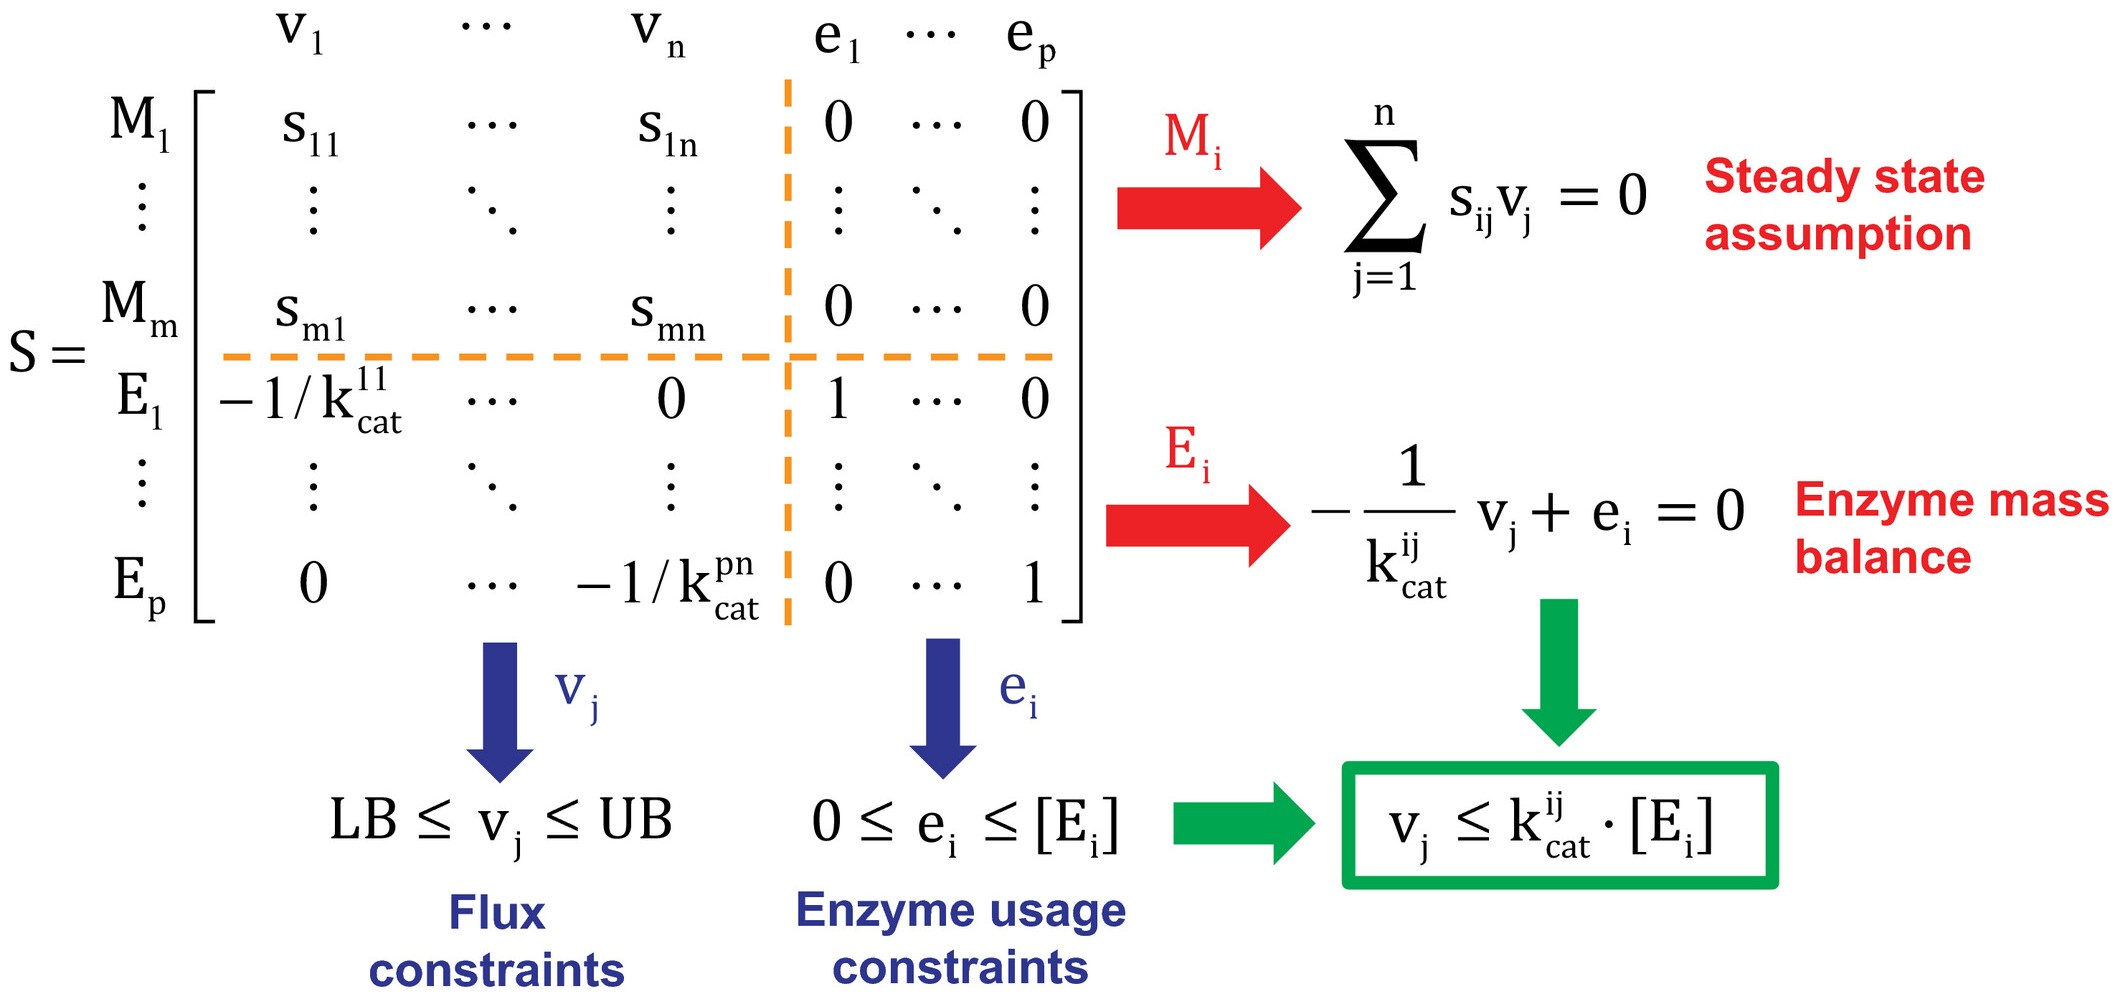
\includegraphics[width=0.8\textwidth]{Images/gecko.jpg}
    \label{fig:gecko}
\end{figure}

\unsure[inline]{what about isozymes etc}
\cite{improving_phenotype_predictions} %GECKO
